\documentclass[12pt]{book}

\usepackage[utf8]{inputenc}
\usepackage[T1]{fontenc}
\usepackage{times}
\usepackage{setspace}
\usepackage{hyperref}
\usepackage{graphicx}
\usepackage{geometry}
\usepackage{eso-pic}
\usepackage{xcolor}

\begin{document}

\frontmatter

% Adjust margins to zero for the title page
\newgeometry{left=0mm, right=0mm, top=0mm, bottom=0mm}

\begin{titlepage}
    \AddToShipoutPicture*{%
        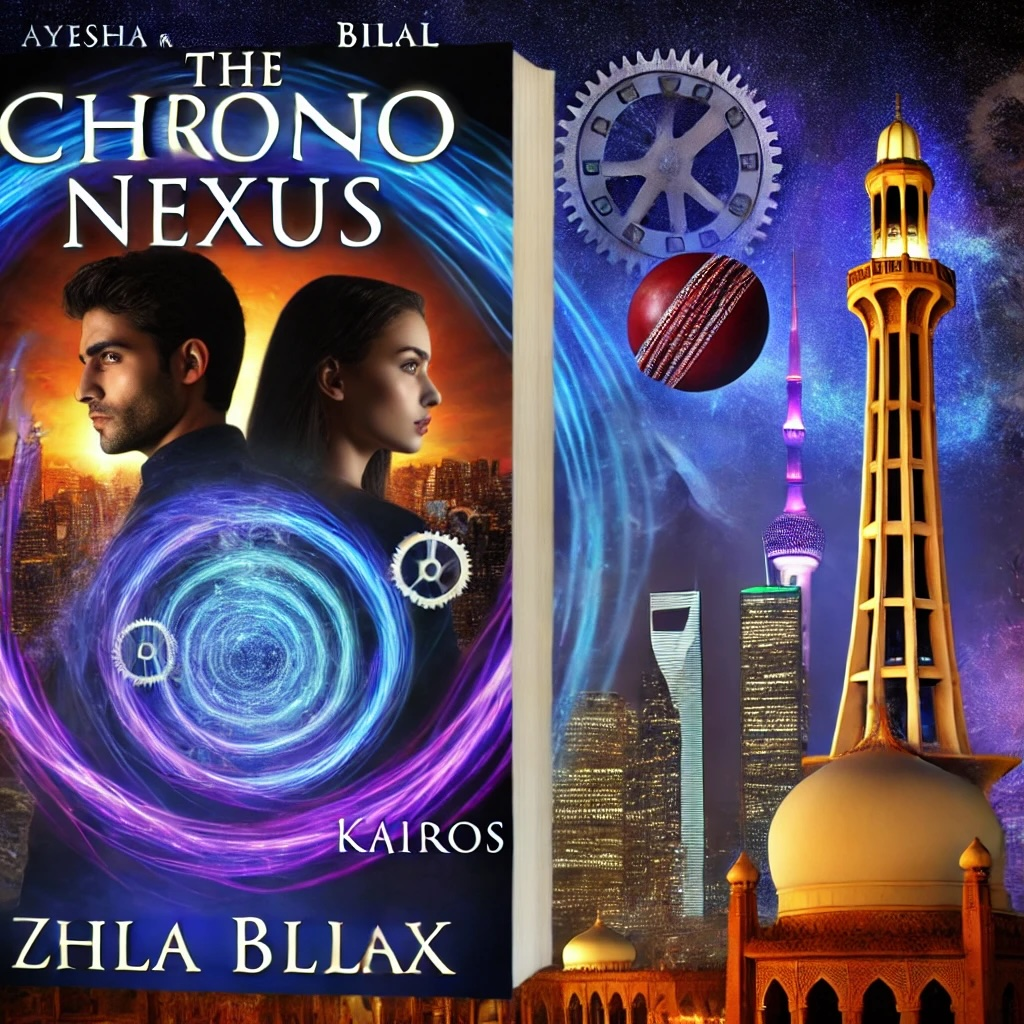
\includegraphics[width=\paperwidth,height=\paperheight]{the_chronos_nexus.jpg}%
    }
    \centering
    \vspace*{5cm} % Adjust vertical spacing as needed
    {\Huge\bfseries\textcolor{white}{The Chrono Nexus}\par}
    \vspace{1cm}
    {\Large\textcolor{white}{A Sci-Fi Thriller}\par}
    \vfill
    {\large\textcolor{white}{By [Your Name]}\par}
    \vspace{2cm}
    {\large\textcolor{white}{\today}\par}
\end{titlepage}

% Restore the original margins for the rest of the document
\restoregeometry

\chapter*{Book Description}
\addcontentsline{toc}{chapter}{Book Description}

\emph{"The Chrono Nexus" is a thrilling sci-fi adventure that follows Ayesha and Bilal, two brilliant young professionals from Lahore, Pakistan. When they discover a time-manipulating device left by Bilal's enigmatic grandfather, they are thrust into a high-stakes mission across global cities like Toronto, Montreal, and New York. Guided by the mysterious time traveler Kairos—who is revealed to be Ayesha's future self—they execute daring heists to dismantle a corrupt syndicate threatening the world's future. Blending sharp wit, suspense, and rich cultural backdrops, the story explores themes of destiny, justice, and the profound impact of courageous individuals on society's course.}

\tableofcontents

\mainmatter

\chapter*{Prologue: Echoes in Time}
\addcontentsline{toc}{chapter}{Prologue: Echoes in Time}

Lahore, Pakistan. The sun dipped below the horizon, casting a golden hue over the sprawling campus of Lahore University of Management Sciences (LUMS). Ayesha navigated the familiar pathways, the evening breeze rustling through the jacaranda trees lining the walkways. She clutched a worn notebook to her chest, her thoughts a whirlwind of uncertainty.

\begin{quote}
    ``Late again, Ayesha?'' called out Bilal, emerging from the shadows of the old library.

    She smiled wryly. ``Some things never change, do they?''

    Bilal chuckled, falling into step beside her. They had been friends since their university days---both brilliant, both restless, both yearning for something more than the hand life had dealt them. Ayesha, with her sharp wit and unyielding spirit, and Bilal, with his charming demeanor and inquisitive mind, found solace in each other's company amid the chaos of their lives.
\end{quote}

As they strolled through the campus, memories of youthful dreams and ambitions surfaced. But those dreams now seemed distant, overshadowed by the harsh realities of financial struggles and a corrupt system that stifled their potential.

\begin{quote}
    ``Remember when we thought we could change the world?'' Ayesha mused, gazing up at the night sky.

    Bilal sighed. ``We were so naive. But maybe... maybe it's not too late.''
\end{quote}

Their footsteps led them to the old physics building, a relic from another era. Bilal paused, his eyes lingering on the weathered façade.

\begin{quote}
    ``There's something I want to show you,'' he said, a hint of excitement in his voice.
\end{quote}

Curiosity piqued, Ayesha followed him inside.

\chapter{The Hidden Legacy}

The attic was a treasure trove of forgotten artifacts. Dust particles danced in the beam of a flashlight as Bilal rummaged through stacks of old books and equipment. Ayesha wrinkled her nose at the musty smell, watching as he unearthed a leather-bound diary from beneath a pile of yellowed manuscripts.

\begin{quote}
    ``This belonged to my grandfather,'' Bilal explained, his eyes alight with anticipation. ``He was a physicist here in the '70s. Disappeared under mysterious circumstances.''

    Ayesha raised an eyebrow. ``And you think this diary holds the key to his disappearance?''

    ``Maybe. Or maybe it's the key to something much bigger.''
\end{quote}

They settled on the creaking floorboards, poring over pages filled with intricate diagrams, complex equations, and cryptic notes.

\begin{quote}
    ``These are... schematics for some kind of device,'' Ayesha murmured, tracing a finger over a detailed drawing.

    ``A device capable of manipulating time,'' Bilal confirmed.

    She shot him a skeptical look. ``Time travel? Seriously?''

    He met her gaze steadily. ``What if we could change things? Make them better?''

    Ayesha hesitated. The allure of such power was intoxicating, but the risks were immeasurable.

    ``Even if this is real, why us?'' she asked softly.

    ``Because we have nothing left to lose,'' Bilal replied. ``And everything to gain.''
\end{quote}

\chapter{Awakening the Past}

Determined to uncover the truth, they followed the diary's instructions to a hidden basement beneath Government College Lahore. The room was a relic of the past, filled with obsolete machinery and faded photographs.

\begin{quote}
    ``Ready?'' Bilal asked, connecting the final wires on a makeshift apparatus.

    Ayesha took a deep breath. ``As I'll ever be.''
\end{quote}

With a flick of a switch, the machine hummed to life. Lights flickered, and the air crackled with energy. Suddenly, a vortex of shimmering light materialized before them.

From within the vortex stepped a figure clad in a sleek, futuristic suit. The stranger removed their helmet, revealing a face that seemed both familiar and foreign.

\begin{quote}
    ``Who are you?'' Ayesha demanded, her heart pounding.

    ``I am Kairos,'' the stranger replied, their voice echoing slightly. ``A traveler from a future that must not come to pass.''

    Bilal exchanged a glance with Ayesha. ``This is impossible.''

    ``On the contrary,'' Kairos said with a faint smile. ``It's inevitable.''
\end{quote}

\chapter{The Proposition}

Over cups of steaming chai in a dimly lit café, Kairos laid out their mission.

\begin{quote}
    ``In my time, the world is on the brink of collapse,'' they explained. ``Corruption and greed have poisoned society. But we can change that.''

    ``You want us to commit crimes to stop crimes?'' Ayesha challenged.

    ``Think of it as rebalancing the scales,'' Kairos countered. ``Targeting key financial institutions linked to corrupt networks. Redirecting funds to where they're needed most.''

    Bilal leaned forward. ``And you need us because...?''

    ``Because you're the only ones who can,'' Kairos said. ``Your grandfather knew this, Bilal. He began this work decades ago.''

    Ayesha contemplated the weight of their words. ``If we agree, what guarantees do we have that this will work?''

    Kairos met her gaze. ``There are no guarantees. Only opportunities.''
\end{quote}

\chapter{Training for the Impossible}

Over the following weeks, Kairos trained them rigorously. In abandoned warehouses and secluded corners of the city, they honed their skills.

Ayesha mastered social engineering, learning to manipulate situations and people with ease. Bilal delved into advanced technology, his background in computer science proving invaluable as he absorbed knowledge of future tech.

They practiced combat techniques, hacking, and stealth operations. Each session pushed them to their limits.

\begin{quote}
    ``Again,'' Kairos insisted as Ayesha struggled to bypass a simulated security system.

    She groaned. ``You're a relentless taskmaster, you know that?''

    Kairos smirked. ``Perfection requires perseverance.''

    Despite the grueling regimen, a camaraderie blossomed among them. Shared jokes in Urdu, playful banter, and moments of vulnerability solidified their partnership.

    ``¿Estás listo para esto?'' Bilal asked one evening, switching to Spanish.

    Ayesha nodded, determination in her eyes. ``We're as ready as we'll ever be.''
\end{quote}

\chapter{The First Heist – Montreal}

Their first target was a bank in Montreal, Canada, known to launder money for corrupt officials.

Using the time device, they arrived in Montreal on a crisp autumn morning. The city buzzed with activity, leaves painted in hues of gold and crimson.

Ayesha adjusted her glasses, her French impeccable as she approached the receptionist.

\begin{quote}
    ``Bonjour, je suis ici pour voir M. Dupont.''

    ``Un moment, s'il vous plaît,'' the receptionist replied politely.
\end{quote}

Meanwhile, Bilal infiltrated the bank's network from a van parked nearby, his fingers dancing over the keyboard.

\begin{quote}
    ``Security systems are down for the next ten minutes,'' he informed her through an earpiece.

    ``Copy that,'' Ayesha whispered, slipping past the receptionist with a forged ID.
\end{quote}

She accessed the vault, planting a device that began siphoning illicit funds into accounts earmarked for humanitarian aid.

\begin{quote}
    ``Time's up,'' Bilal warned.

    A security guard approached, suspicion in his eyes. ``Madame, vous ne devriez pas être ici.''

    Thinking quickly, Ayesha feigned distress. ``Oh, je suis désolée! Je me suis perdue en cherchant les toilettes.''

    The guard relaxed slightly. ``C'est au deuxième étage.''

    ``Merci beaucoup,'' she said with a disarming smile.
\end{quote}

Rejoining Bilal, they slipped away unnoticed, the first mission a resounding success.

\chapter{Unveiling the Network}

Back in Lahore, Kairos reviewed the data they had acquired.

\begin{quote}
    ``With this, we can disrupt a significant portion of the syndicate's operations,'' they said.

    Bilal nodded. ``But they'll notice the missing funds eventually.''

    ``That's why we have to keep moving,'' Ayesha asserted. ``Hit them where they least expect it.''
\end{quote}

Their next targets took them to Toronto and Quebec City. In Toronto, they charmed their way into exclusive circles, gathering intel and accessing restricted systems. In Quebec City, they staged a protest against healthcare cuts—a cause close to Ayesha's heart—creating a diversion while Bilal extracted vital information.

Each success emboldened them, but the stakes grew higher.

\chapter{The Thompson Encounter}

In the remote town of Thompson, Manitoba, they faced unforeseen challenges. The bank was heavily fortified, and the cold was bone-chilling.

\begin{quote}
    ``Reminds me of Murree in winter,'' Bilal joked, his breath forming clouds.

    ``Focus,'' Ayesha admonished, though a smile tugged at her lips.
\end{quote}

Using advanced technology, they bypassed the security systems. But as they made their escape, alarms blared.

\begin{quote}
    ``Looks like they've upgraded,'' Bilal muttered.

    They sprinted through icy streets, pursued by security personnel.

    ``This way!'' A voice beckoned from an alley.

    Ayesha hesitated. ``Can we trust him?''

    ``We don't have a choice,'' Bilal replied.
\end{quote}

They followed the stranger into a hidden passage.

\begin{quote}
    ``You're lucky I found you,'' he said in accented English. ``Name's Carlos. Kairos sent me.''
\end{quote}

\chapter{Allies and Adversaries}

Carlos, a Spanish ex-pat fluent in Urdu and Spanish, joined their team as an expert in logistics.

\begin{quote}
    ``Mi casa es su casa,'' he quipped, offering them shelter.
\end{quote}

With his help, they expanded their operations, reaching as far as San Diego and Phoenix, Arizona. Each heist was a carefully orchestrated symphony of precision and daring.

But shadows lurked on the horizon. Reports surfaced of an elusive group targeting banks worldwide. The syndicate began tightening its grip, employing ruthless tactics to protect their interests.

In New York City, they encountered Sofia, a psychology lecturer and master of social engineering. Her insights proved invaluable, but she warned them of the dangers ahead.

\begin{quote}
    ``You're playing a dangerous game,'' she cautioned over dinner in a cozy Brooklyn café.

    ``Change never comes without risk,'' Ayesha countered.

    Sofia smiled knowingly. ``Just be careful. The higher you climb, the harder you fall.''
\end{quote}

\chapter{The Princeton Revelation}

In Princeton, New Jersey, they sought the assistance of Dr. Amir, an oncologist researching cancer treatments halted due to lack of funding—a direct consequence of the syndicate's actions.

Dr. Amir greeted them warmly.

\begin{quote}
    ``I've heard of your endeavors. You're making waves.''

    ``We need access to the university's archives,'' Bilal explained. ``There might be information linking the syndicate to political figures.''

    Dr. Amir agreed, but as they delved deeper, they uncovered a startling connection—the syndicate had ties to high-ranking officials in Pakistan's government and military.

    ``This goes all the way to the top,'' Ayesha whispered, her hands trembling.

    Bilal clenched his fists. ``We have to expose them.''

    But Kairos intervened. ``It's too dangerous. You're not ready for this level of exposure.''

    Ayesha bristled. ``People are suffering. We can't just stand by.''

    Kairos's expression was unreadable. ``There are consequences you don't understand.''
\end{quote}

\chapter{Betrayal and Truth}

Tensions mounted within the team. Trust wavered as secrets surfaced.

One night in a secluded motel, Ayesha confronted Kairos.

\begin{quote}
    ``You're hiding something,'' she accused. ``Who are you really?''

    Kairos sighed heavily. ``You deserve the truth.''
\end{quote}

Removing their helmet, Kairos revealed a familiar face—Ayesha's own, etched with lines of age and sorrow.

\begin{quote}
    Ayesha staggered back. ``This... this can't be.''

    ``I'm you,'' Kairos confirmed. ``From a future ravaged by the syndicate's actions.''

    Bilal stared in disbelief. ``Why didn't you tell us?''

    ``Because knowing your future can be a burden,'' Kairos replied. ``I wanted to spare you that.''

    Ayesha grappled with the revelation. ``All this time... I was following myself?''

    Kairos placed a hand on her shoulder. ``I knew you could succeed where I failed.''
\end{quote}

\chapter{The Final Heist}

Determined to end the syndicate's reign, they planned their most ambitious heist yet—a bank in New York City serving as the syndicate's central hub.

Using every skill they had acquired, they infiltrated the heavily guarded facility. Ayesha and Bilal navigated laser grids and biometric scanners, their movements synchronized flawlessly.

\begin{quote}
    ``Remember, we have a narrow window,'' Kairos reminded them over the comms.

    They reached the central server room, uploading a virus designed to expose the syndicate's operations to international authorities.

    ``Data transfer at 80\%,'' Bilal reported.

    Suddenly, the doors locked down. Red lights flashed.

    ``Security breach detected,'' an automated voice announced.

    ``We've been compromised,'' Ayesha hissed.

    ``Hold your position,'' Kairos ordered. ``I'm initiating a diversion.''

    Explosions rocked the building's exterior, triggering panic.

    ``Transfer complete!'' Bilal exclaimed.

    They fought their way out, evading armed guards. Just as they reached the exit, an agent cornered them.

    ``End of the line,'' he sneered.

    Before he could act, a shot rang out. The agent fell, revealing Captain Malik—a Pakistani army officer committed to justice.

    ``Time to go,'' he urged.
\end{quote}

\chapter{Sacrifice and Farewell}

Outside, chaos reigned as emergency services swarmed.

\begin{quote}
    ``Get to the extraction point,'' Kairos instructed.

    They raced to a rooftop where a helicopter awaited, piloted by Carlos.

    ``¡Vámonos!'' he shouted.

    As they lifted off, Kairos remained behind.

    ``You're not coming?'' Ayesha asked urgently.

    Kairos shook her head. ``My time here is done. The future is in your hands now.''

    Tears welled in Ayesha's eyes. ``Thank you... for everything.''

    Kairos smiled softly. ``Live well, and make different choices.''
\end{quote}

With that, the helicopter soared into the night, leaving Kairos fading into the shadows.

\chapter{A New Dawn}

Back in Lahore, life began to change. News outlets reported mass arrests of corrupt officials. Funds were redistributed to healthcare, education, and social programs.

Dr. Amir's cancer research received substantial backing, leading to groundbreaking developments.

Ayesha and Bilal established a foundation supporting mental health initiatives, honoring Ayesha's late mother.

One evening, they attended a cricket match at Gaddafi Stadium. The crowd's energy was electric, uniting people from all walks of life.

\begin{quote}
    ``Look at them,'' Ayesha said, her heart swelling with hope. ``This is what it's all about.''

    Bilal nodded. ``We did good, didn't we?''

    She smiled. ``Yeah, we did.''
\end{quote}

\chapter*{Epilogue: Threads Through Time}
\addcontentsline{toc}{chapter}{Epilogue: Threads Through Time}

Months later, Ayesha visited the old café where she first met Kairos. As she sipped her chai, a familiar figure slid into the seat across from her.

\begin{quote}
    ``Long time no see,'' Sofia greeted.

    Ayesha grinned. ``To what do I owe the pleasure?''

    Sofia leaned in conspiratorially. ``I've been hearing whispers. Seems our work isn't finished.''

    Ayesha arched an eyebrow. ``What do you have in mind?''

    Sofia placed a small device on the table---a time manipulator similar to Kairos's.

    ``Interested in one more adventure?''

    Ayesha considered the device, memories of past exploits flickering in her mind.

    She picked it up, a determined gleam in her eyes. ``\textit{Siempre}.''

    Together, they stepped into the unknown, ready to weave new threads through the tapestry of time.
\end{quote}

\backmatter

% Optional: You can add acknowledgments, about the author, or other back matter here.

\end{document}
